\documentclass[preprint]{aastex}

% packages for figures
\usepackage{graphicx}
% packages for symbols
\usepackage{latexsym,amssymb,hyperref}
% AMS-LaTeX package for e.g. subequations
\usepackage{amsmath}

%=====================================================================
% FRONT MATTER
%=====================================================================

\slugcomment{Draft \today}

%=====================================================================
% BEGIN DOCUMENT
%=====================================================================

\newcommand{\kmax}{\ensuremath{k_\mathrm{max}}}
\newcommand{\kmin}{\ensuremath{k_\mathrm{min}}}
\newcommand{\rmd}{\ensuremath{\mathrm{d}}}
\newcommand{\beq}{\begin{equation}}
\newcommand{\eeq}{\end{equation}}

\begin{document}

\title{Lensing engine testing and normalization convention (Issue \#248)}

\begin{abstract}
This document contains Rachel's notes on tests of the lensing engine
for GalSim Issue \#248.  There are a number of questions we need to
check to make sure that that software is doing what we want it to do,
and all the relevant tests and equations are described below.
\end{abstract}

\section{Introduction}

There are a few issues that we wish to check regarding the lensing
engine.  They are:

\begin{enumerate}
\item Overall normalization of shear variance: Currently the shear
  variance for a constant input shear power does not depend on
  the grid size/shape.  This seems non-standard, so we should
  investigate and understand this further.
\item We need to check the scaling of either the observed correlation
  function or power spectrum with $k$, to make sure it is done right.
\item What is the effect of interpolating between grid points?  does
  the interpolant have the expected impact on the shear power?
\item If we put in just $E$ or just $B$ mode power with a flat
  spectrum, the variances of $\gamma_1^2$ and $\gamma_2^2$ differ; is
  this expected for a flat power spectrum or sign of a problem?
\item We should make sure that when we use both $E$ and $B$ mode
  power, that we get the expected result, and that results with only
  $E$ or only $B$ are also sane.
\item Impact of differences between continuous vs. discrete
  representation?
\end{enumerate}

\section{Theory}

The lensing engine requires a shear power spectrum, $P(k)$.  We are
working in the flat-sky limit, so when we see expressions in terms of
$\ell$ we can swap $\ell$ with $k$ and $C_\ell$ with $P$, and
\beq
\Delta^2 = \frac{\ell(\ell+1) C_{\ell}}{2\pi}\equiv \frac{k^2 P(k)}{2\pi}.
\eeq
When people plot shear power spectra they usually actually plot
$\Delta^2(k)$ (or, in terms of the full-sky formalism, they plot $\ell(\ell+1)C_\ell/(2\pi)$).

If we identify pairs of galaxies and get the shears in a coordinate
system defined along the vector connecting them ($\gamma_+$) and at 45
degrees with respect to it ($\gamma_\times$), then we can compute
correlation functions of the $\gamma_+$ and $\gamma_\times$ values,
which we will call $\xi_{++}$ and $\xi_{\times\times}$.  Then the
standard cosmological correlation functions $\xi_{\pm}$ are defined as
\begin{align}
\xi_{\pm}(\theta) &=  \xi_{++}\pm \xi_{xx} \\
 &= \frac{1}{2\pi}\int k\,\rmd k P(k) J_{0/4}(k\theta).
\end{align}

Since correlation functions are dimensionless, we immediately see that
$P(k)$ has dimensions of angle$^2$ and $\Delta^2(k)$ is dimensionless.

The variance of the shear values, 
\beq
\mathrm{Var}(\gamma) = \langle g_1^2 + g_2^2\rangle,
\eeq
is essentially $\xi_+(\theta=0)$.   Note that this is what we get for
the defined $\xi_+$ in the limit of $\theta$ going to zero, but that
equation was defined in terms of $\gamma_+$ and $\gamma_\times$ rather
than $\gamma_1$ and $\gamma_2$.  On a grid, it's not clear that we
can enforce/check behavior of Var($\gamma_1$) or Var($\gamma_2)$,
particularly if the corners are important (which will be the case if
there is a lot of shear power at small $k$), probably we should 
 only expect normal behavior for Var($\gamma$), but it's still worth
 verifying this.  So, combining several equations,
\beq\label{E:shearvar}
\mathrm{Var}(\gamma) = \frac{1}{2\pi}\int k\,\rmd k P(k).
\eeq
which essentially says the shear variance is the power integrated over
the allowed area in $k$ space.  I {\em think} that if we want to work
in terms of $k_x$ and $k_y$, we can replace $2\pi k\rmd k$
(integrating within a circle) with $\rmd
k_x \rmd k_y$ (integrating within our square grid), so the above might also be
written as
\beq\label{E:alt-shearvar}
\mathrm{Var}(\gamma) = \frac{1}{(2\pi)^2} \int \rmd k_x \rmd k_y
P(k_x, k_y).
\eeq

None of these integrals have had limits on them.  Formally they should
go from the minimum to the maximum accessible $k$ on our grid.  Our
grid is defined by
\begin{align}
L &= \mbox{length of grid along one dimension (angular units)}\\
d &= \mbox{spacing between grid points (angular units)}\\
N &= \mbox{number of grid points along one dimension} = L/d
\end{align}

In all of the above I have simply written $P(k)$ but in principle there can be
two such functions, $P_{E}$ and $P_B$.  I believe these
should simply be summed in the above variance equation, but should check this.

A note about something possibly confusing: there are many papers that
write equations for shear variances that include some window function,
which we haven't included here.  I believe that is okay, because those
papers are referring to a different calculation: they are averaging
the shear in some cells, and computing the expected variance of those
shears that have been averaged in cells.  In contrast, we're computing
the variance of individual shears that have been defined within our
grid, which is a completely different thing.

\section{Comparison software}

We will compare against a completely independent piece of software,
Chris Hirata's spherical harmonic transform code which is described in
multiple papers (for example,
\href{http://adsabs.harvard.edu/abs/2004PhRvD..70j3501H}{Hirata
  et~al. 2004}).  This does not use the flat-sky
approach, but that should not be huge important of a difference even
for our $L=10$ deg.  It is something to bear in mind if we start
looking for agreement at a few \% level on the largest $\theta$ or
smallest $k$.  This software wants $C_\ell(\ell)$ as its inputs.

\section{General considerations for these tests}

First, it's not clear that we should really be enforcing $P(0)=0$,
i.e., no power below our \kmin.
This is a valid condition for the full-sky power spectrum, but will
not in general be valid for a small patch of the sky, due to sampling
variance.  In order to include this sampling variance, it would be
preferable to assign $P(0)=$ some kind of integral over $P(k<\kmin)$
(perhaps an average power in that $k$ range; details to be worked out later) assuming the power function is
defined for those value of $k$.

Second, since we use a DFT of a finite set of samples, we implicitly
have a $k$ defined on a periodic grid, not simply $k=0$ for all
$k>\kmax$.  This also means that we should possibly avoid using the
variance as a metric, because what we really care about is whether the
PS is represented properly within our $k$ range.

Moreover, we need to be well-sampled in $k$ space, so we should not
use functions that do unreasonable things like $k^{-2}$.

Barney suggested a test case that is a Gaussian, i.e., $P(k) =
e^{-\sigma^2 k^2 / 2}$, so $\xi_+(\theta) =
e^{-\theta^2/2\sigma^2}/(2 \pi \sigma^2)$ and the variance may be
$\xi_+(0)=1/(2\pi\sigma^2)$.  I will define the Gaussian such that
there is essentially no power left at our \kmax, which is
$2\pi/d=0.0175$ arcsec$^{-1}$.  Let's use $\sigma \kmax=5$ or
$\sigma=286.5$ arcsec for the first two grids, $\sigma=573.0$ for the
third grid.  The code is:
\begin{verbatim}
import galsim
import numpy as np
test_ps = galsim.PowerSpectrum(lambda k : np.exp(-0.5*((286.5*k)**2)))
g1, g2 = test_ps.buildGriddedShears(grid_spacing=360., ngrid=100)
print np.var(g1), np.var(g2), np.var(g1)+np.var(g2)
g1, g2 = test_ps.buildGriddedShears(grid_spacing=360., ngrid=50)
print np.var(g1), np.var(g2), np.var(g1)+np.var(g2)
test_ps = galsim.PowerSpectrum(lambda k : np.exp(-0.5*((573.0*k)**2)))
g1, g2 = test_ps.buildGriddedShears(grid_spacing=720., ngrid=50)
print np.var(g1), np.var(g2), np.var(g1)+np.var(g2)
\end{verbatim}

The result is the same variance in each case (and the same for each
component, unlike many of our other test cases which had different
variances for the two components), around 0.24.  This is not the value
that I expected numerically, but it at least means we understand the
grid-dependence of the result, since my change in $\sigma$ for the
last grid correctly preserved the variance despite the different grid
spacing.  Moreover the variance doesn't depend significantly on \kmin,
as predicted.

\section{Test of $P(k)$}\label{S:testpk}

I have a WMAP7 LCDM prediction for the cosmic shear signal for a
sample with $z_{med}\sim 0.55$, which I can use as an input to both
the SHT code and ours.  Given the range of $\ell$ for which it is
defined, $2<\ell<2000$, we cannot use our standard grid because that
has $\kmax=3600$ radians$^{-1}$.  So, for this test I use a grid with
the same $L$ as before, but $N=50$ (i.e., $d$ gets doubled), which
means $\kmax=1800$ radians$^{-1}$.

Using the SHT code, I made gridded shears for each of 3 cases:
$P_E=P(k)$ and $P_B=0$; $P_B=P(k)$ and $P_E=0$; and $P_E=P_B=P(k)$ (5
realizations of each).
For GalSim, since it's less computationally expensive I averaged over
more realizations; for our code, it is crucial to inform the code that
the inputs have units of radians.

The python script test\_pk.py in devel/external/test\_gridshear/ does the following:
\begin{enumerate}
\item Generates shears according to this PS using GalSim.
\item Runs the GREAT10 power spectrum code on both (must flip sign of
  one shear component before doing so), and averages it over several
  noise realizations.
\end{enumerate}

The python script test\_pk\_sht.py in that directory does the following:
\begin{enumerate}
\item Manipulate outputs of the SHT code to be consistent with
  expectations (incl. one sign flip for e1).
\item Runs the GREAT10 power spectrum code on it.
\end{enumerate}

Finally, plot\_pk\_test.py in that directory plots the original and
simulated $P(k)$ based on these files.  The results for the three
cases (input $P_E$, input $P_B$, and input $P_E=P_B$) are in
Figures~\ref{F:pe}, \ref{F:pb}, \ref{F:peb}.

\begin{figure}
\begin{center}
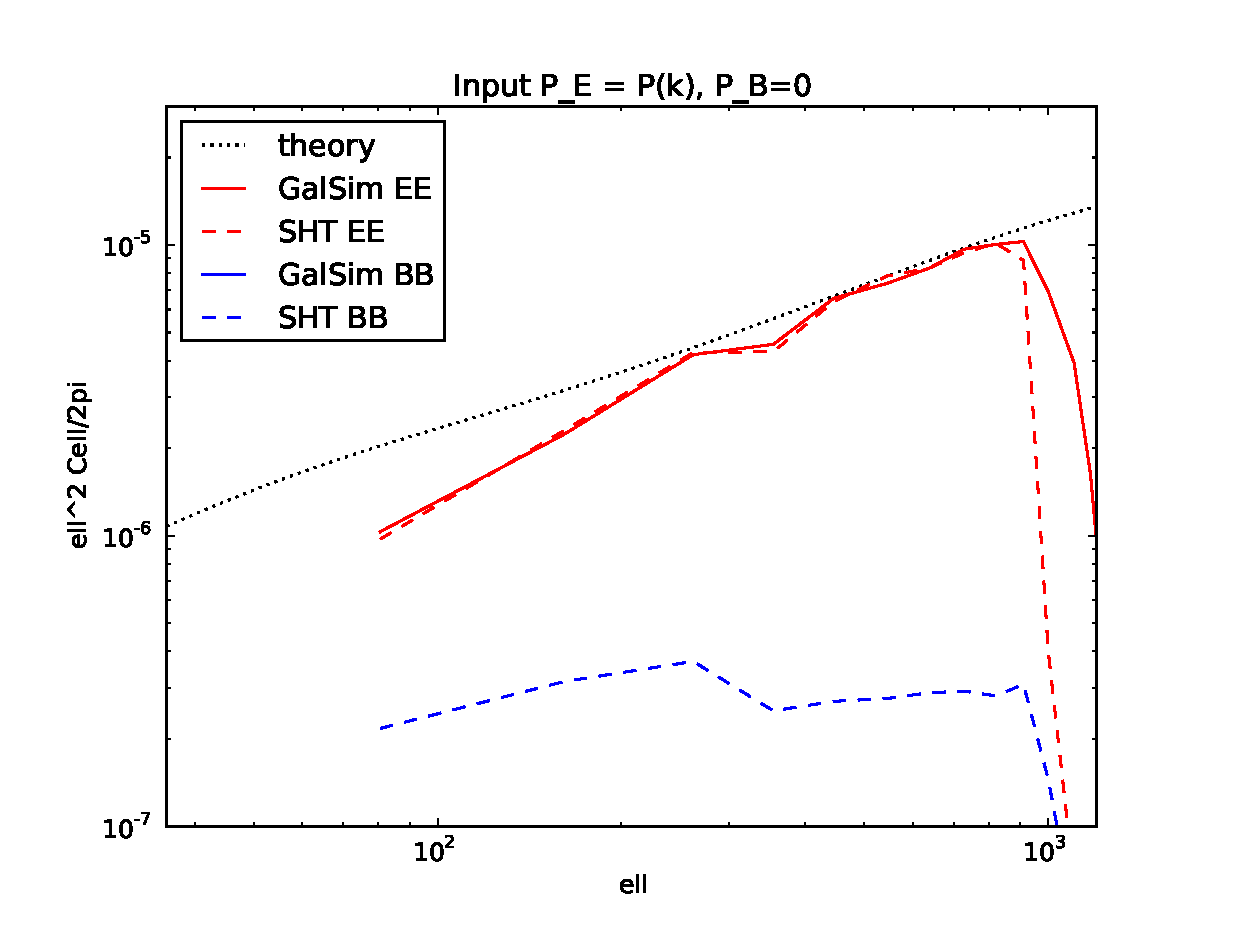
\includegraphics[width=3in]{../external/test_gridshear/output/compare_input_pe.eps}
\caption{Output shear power spectra (plotted as the dimensionless
  $\Delta^2$) for the grids described in Sec.~\ref{S:testpk}, where
  the input $P_E$ is a realistic cosmological one (shown as the 'theory' line on
  the plot) and the input $P_B=0$. The results for GalSim and the
  comparison SHT code are both plotted.\label{F:pe}}
\end{center}
\end{figure}

\begin{figure}
\begin{center}
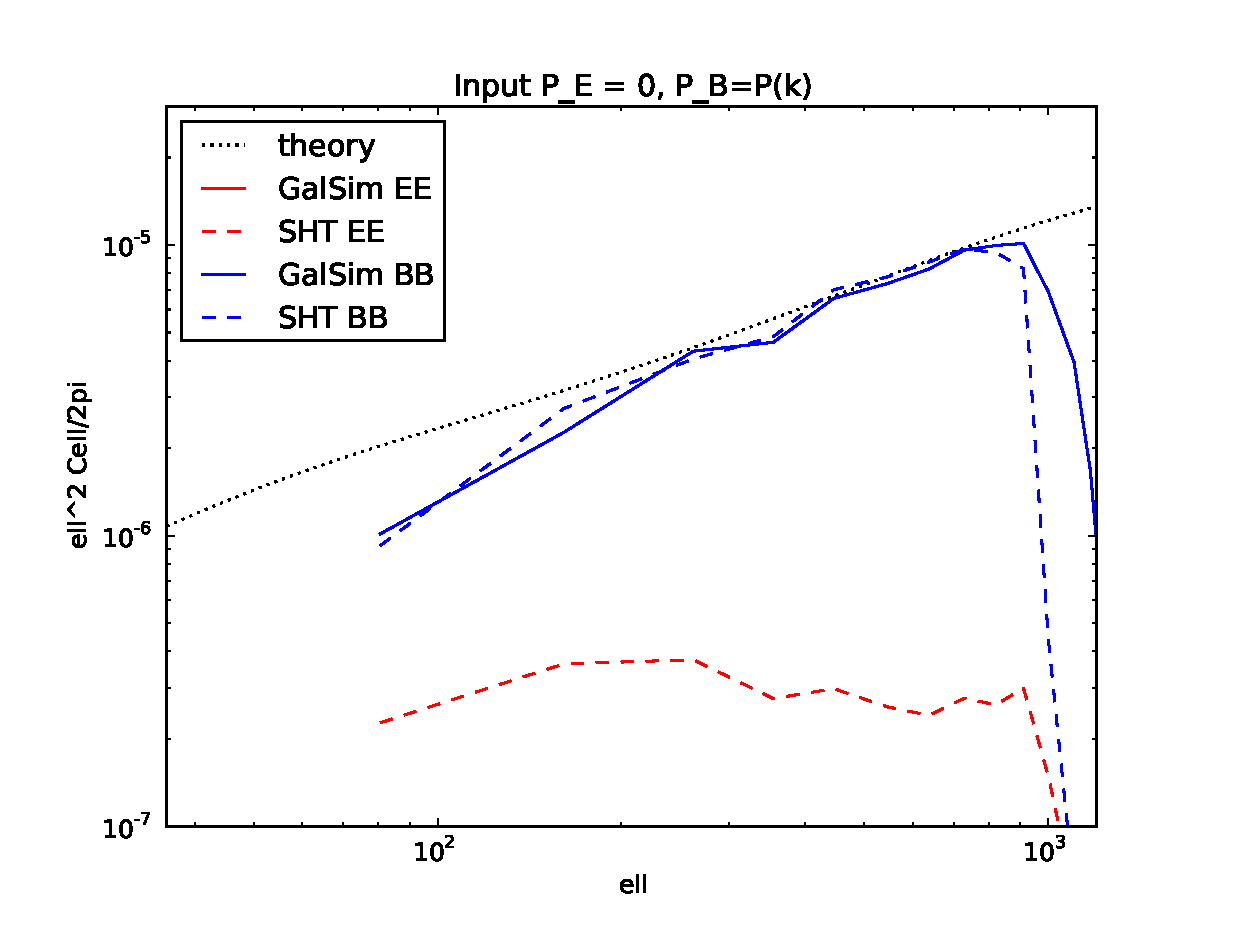
\includegraphics[width=3in]{../external/test_gridshear/output/compare_input_pb.eps}
\caption{Output shear power spectra (plotted as the dimensionless
  $\Delta^2$) for the grids described in Sec.~\ref{S:testpk}, where
  the input $P_B$ is a theoretical one and the input $P_E=0$. The results for GalSim and the
  comparison SHT code are both plotted.\label{F:pb}}
\end{center}
\end{figure}

\begin{figure}
\begin{center}
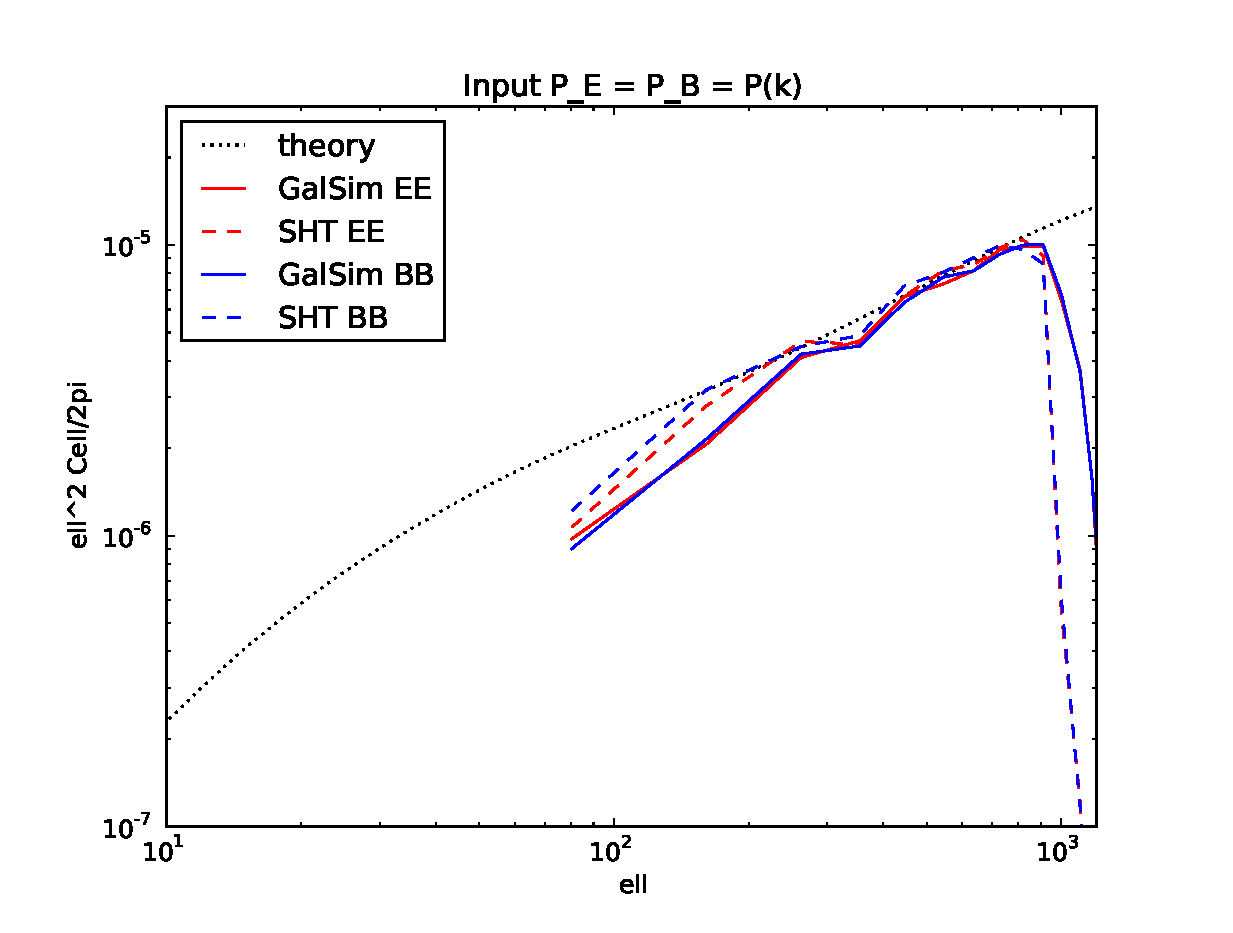
\includegraphics[width=3in]{../external/test_gridshear/output/compare_input_peb.eps}
\caption{Output shear power spectra (plotted as the dimensionless
  $\Delta^2$) for the grids described in Sec.~\ref{S:testpk}, where
  the input $P_E=P_B$ is shown as the 'theory' line. The results for GalSim and the
  comparison SHT code are both plotted.\label{F:peb}}
\end{center}
\end{figure}

Conclusions:
\begin{itemize}
\item SHT code: it gives roughly a consistent power spectrum compared
  to our inputs (modulo possible slight differences in scaling that
  may not be worth investigating until our own PS code is ready),
  though there are signs of $E$ vs. $B$ leakage in the case where one
  or the other is zero.
\item GalSim: we don't see $E$ vs. $B$ leakage at any significant
  level, but the amplitudes are consistently too high by $\sim 4\times
  10^6$.  The scaling with $\ell$ is about right.
\end{itemize}

I am not sure where this amplitude offset could come from.  There are
several large numbers that come into these calculations, e.g., there
is the radians vs. arcsec conversion which is $\sim 2\times 10^5$,
and there is the grid $N^2=2500$.  To check
for possible dependence on grid $N$, which can sometimes show up if
we've gotten something wrong about the FFT normalization conventions, I reran with the same $d$ but
with $L$ and $N$ halved (5 degree grid, 0.2 degrees between grid
points, $N$=25).  The results did not change (modulo a bit more noise
as expected since there are fewer pairs of grid points with which to
measure the power).  So I think it must be some other factor somewhere.
\begin{figure}
\begin{center}
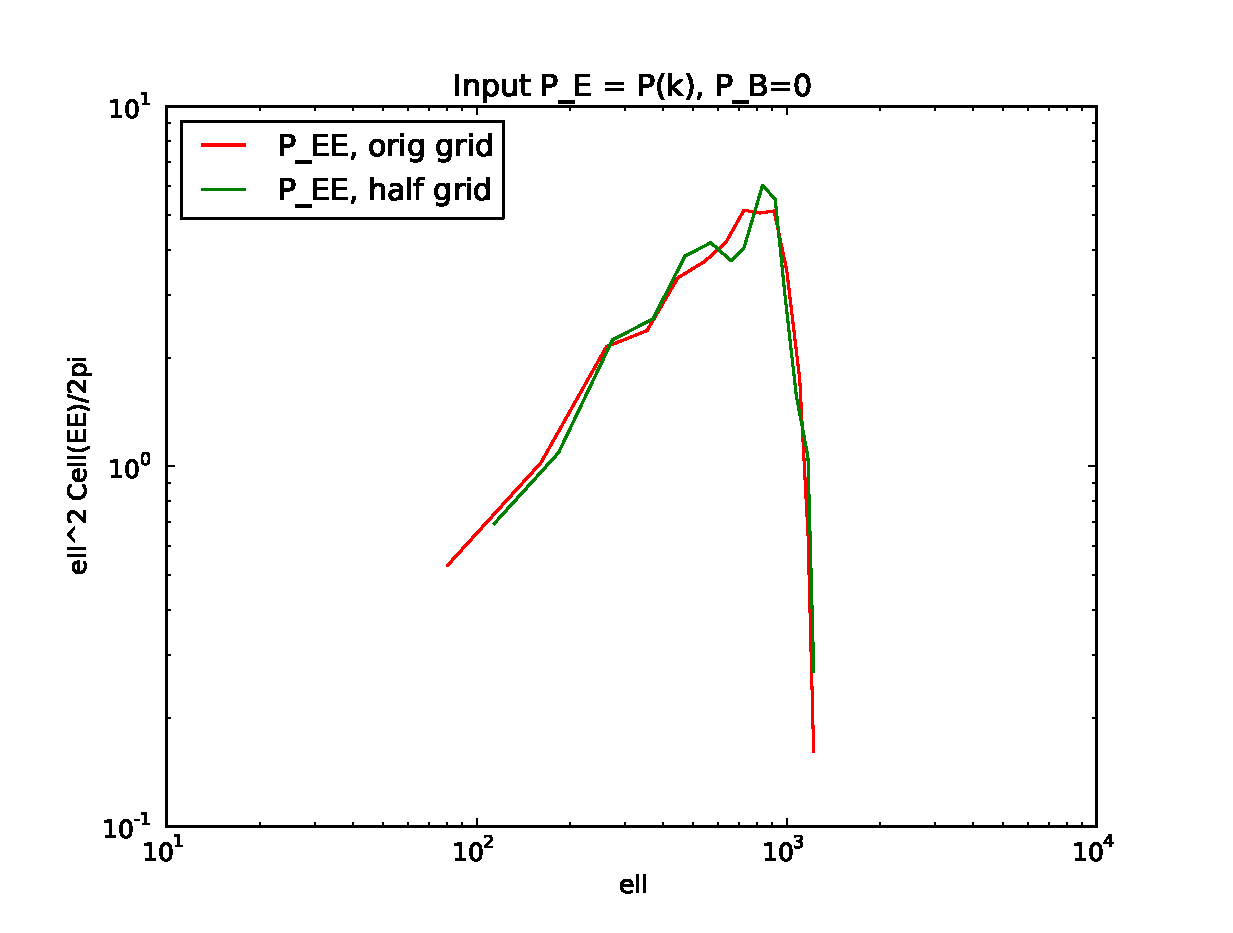
\includegraphics[width=3in]{../external/test_gridshear/output/compare_input_pe_halfn.eps}
\caption{Output shear power spectra (plotted as the dimensionless
  $\Delta^2$) for the grids described in Sec.~\ref{S:testpk} and for
  one that covers half the linear extent ($1/4$ the area).  Both
  results are for GalSim, comparing the previous grid with this one.\label{F:pe_halfn}}
\end{center}
\end{figure}

I did a sanity check of the numbers that the lensing engine used when
finding the power for each $k$ on the grid.  The grid has a $\Delta
k_x=\Delta k_y = 0.00017453$.  We expected $2\pi/(10\times 3600)$
arcsec$^{-1}$, so this is correct.  That corresponds to $36$
radians$^{-1}$, so the power at that $k$ should be $5.23\times 10^{-9}$
radians$^2$, which is $2.23\times 10^{2}$ arcsec$^2$.  That is the
number that GalSim gives for $k_x=\kmin$ and $k_y=0$ (and vice versa),
so it seems we've done the most basic part of the units conversions
right.

\end{document}
